\documentclass[conference]{IEEEtran}
\usepackage{amsmath}
\usepackage{booktabs}
\usepackage{graphicx}
\newcommand{\ParentCaseCount}{2,279}
\newcommand{\AuditModelCount}{2,317}
\newcommand{\ParentApplicability}{98.4\%}


\title{Where Should Provenance Policy Run? A Comparison of On-Chain Enforcement and Attested Model Lineage}
\author{\IEEEauthorblockN{Author names to be confirmed}
\IEEEauthorblockA{CSCI 435 Research Track}}

\begin{document}
\maketitle

\begin{abstract}
We compare three EVM designs for auditing model ancestry on a workload
derived from a Hugging Face model family. A direct storage registry
records parent links. A second registry enforces provenance policy in
Solidity. A third evaluates the policy off-chain and anchors attested
Merkle commitments. On local Anvil replays, batching reduces
registration gas and new on-chain storage. Synthetic chains and
multi-parent records show that storage-based verification costs grow
with lineage complexity, while the anchored target check remains
roughly constant at batch size one. Controlled tests distinguish inputs
refused by admission policy from alterations detected during an audit.
The anchored design relies on the attester and on access to the
off-chain records and proofs.
\end{abstract}


\section{Introduction}
A model published on a public hub may derive from one checkpoint or merge
several checkpoints. An auditor tracing a released model needs to recover
those relationships and identify which provenance checks applied when the
record was published. We ask how three EVM registry designs compare in
registration gas and storage, lineage verification latency and throughput,
and their handling of invalid registrations and changed audit inputs. The comparison addresses
three questions:
\begin{enumerate}
  \item How do registration gas and newly occupied state change with
  the provenance design, lineage depth, and number of parents?
  \item What does it cost to evaluate the policy and verify a lineage,
  and how many records can one auditor verify per second?
  \item Which controlled invalid inputs fail at admission, and which
  changes to a committed record are detected during an audit?
\end{enumerate}

\section{Background and Related Work}
% Authors: write this section from the assigned Moodle readings and papers
% you have read. Add verified BibTeX entries and connect the gap to that work.

\section{Registry Designs}
D1 stores the publisher's model record, the first version, and the parent
model IDs in Solidity storage. Each parent must already have a registered
version. Parent edges are fixed at model registration and identify the
parents' first versions for the benchmark. Subsequent versions keep the
model's parent edges and can only be appended by its current owner. D2
adds checks for parent revocation, duplicate weights, approved dataset
references, a publisher role, and compatibility of declared licence
classes under the experimental policy.

D3 evaluates the D2 policy in Open Policy Agent (OPA). The attester
maintains the parent and weight index and submits an attestation over each
approved batch root. A node hash is SHA-256 over its weight and dataset
reference hashes, the sorted hashes of its parent nodes, and its metadata
hash. The batch leaf commits to the node hash and its publisher address.
The typed attestation binds the batch ID, root, size, and submitter to a
specific chain and contract. An auditor recomputes the ancestry and
checks the target node's inclusion and the associated batch signature.

\subsection{Policy and trust assumptions}
Both enforcement paths require registered, non-revoked parents, nonzero
weight and dataset-reference hashes, unique weight commitments, approved
dataset-reference hashes, an authorized publisher, and a compatible
licence class for each parent. The allowlist and publisher membership
for the replay are derived from the committed registration plan. The
licence compatibility classes are a rule of the experiment, and the
prototype receives the declared class as part of the input. D3 relies
on an authorized attester to maintain the accepted index and apply the
policy. The chain checks the attestation over the commitment.

\section{Evaluation Method}
The benchmark uses the committed 17 November 2026 snapshot of
\texttt{TinyLlama-1.1B-Chat-v1.0} and its Hugging Face descendants.
The pull recorded 2,630 models including 44 external roots. The main
replay contains 2,317 parents-first records after exclusions, 62 of which
have multiple parents. The eligible records reach depth 3. Separate
synthetic workloads cover depths 1--20 and fan-in of 1, 2, 4, and 8.
The commands and data behind these counts are in the repository.

Each design starts on a fresh local Anvil chain with the Cancun hard fork
and a contract compiled with Solidity 0.8.24 and 200 optimizer runs.
The benchmark tests D3 at batch capacities of 1, 16, and 128. Receipts
provide transaction gas and storage traces count newly occupied
32-byte slots. For D3, per-model cost divides a batch transaction's
cost by the actual model count in that transaction. Policy latency is
measured before registration, and lineage latency after registration,
using five warm-up calls and thirty measured calls for each sampled
record. D1 and D2 batch the read requests within each target verification.
Audit throughput is based on five sequential passes over the workload.
Deployment and policy setup are recorded as distinct operations.
Registration gas excludes these two costs. A change from zero to nonzero
in a registry storage slot counts as 32 newly occupied bytes. The
in-contract verification probe measures the lineage query for D1 and
D2 and the inclusion and signature checks for D3. The end-to-end timing
also includes the off-chain work. The verifier uses records already
available to the local process and the experiment does not time file
downloads.

The controlled audit tests present each verifier with the original record
and variants that change its weight or dataset commitment. The parent
variant substitutes an earlier registered record that is absent from the
original parent set. It applies to records with a parent and an available
substitute. The admission tests use the same seeded sample in every
configuration. Each candidate has a fresh weight hash and varies one
condition at a time. D1 and D2 simulate registration with
\texttt{eth\_call}. D3 queries the attester's OPA decision. The tables
count completed decisions, and the generator checks that every planned
candidate has exactly one result.

\section{Results}
% Insert script-generated tables and figures after confirming the run
% manifests. Present receipt gas, off-chain time, and Iris results separately.
\begin{table}[t]
\centering
\caption{Anvil registration cost on the full TinyLlama workload. Gas and
new state are means per model. Setup and deployment are reported
separately in the repository.}
\label{tab:registration}
\begin{tabular}{lrrr}
\toprule
Design & Tx count & Gas/model & Bytes/model \\
\midrule
D1 & 2,317 & 571,877 & 746.7 \\
D2 & 2,317 & 614,533 & 792.4 \\
D3 ($k=1$) & 2,317 & 79,603 & 64.0 \\
D3 ($k=16$) & 145 & 4,989 & 4.0 \\
D3 ($k=128$) & 19 & 660 & 0.5 \\
\bottomrule

\end{tabular}
\end{table}

\begin{table}[t]
\centering
\caption{Median local timing and throughput on the full TinyLlama
workload. D1 has no separate policy measurement.}
\label{tab:timing}
\begin{tabular}{lrrr}
\toprule
Design & Policy (ms) & Verify (ms) & Audit (models/s) \\
\midrule
D1 & -- & 19.90 & 80.27 \\
D2 & 4.67 & 18.80 & 75.17 \\
D3 ($k=1$) & 0.95 & 4.98 & 192.14 \\
D3 ($k=16$) & 0.82 & 4.77 & 212.30 \\
D3 ($k=128$) & 0.73 & 4.59 & 209.43 \\
\bottomrule

\end{tabular}
\end{table}

Table~\ref{tab:registration} compares the same registration workload
across five configurations. D2 adds policy state and checks to the
direct registry. D3 stores one commitment and a compact batch record per
transaction. A larger batch spreads that transaction and state cost
across more models. The batch approach moves policy evaluation and the
record index to the attester. These results measure the on-chain costs
of the implemented designs under the stated trust assumptions.
New state per model is amortized across models in an anchored batch.

Table~\ref{tab:timing} reports the median policy and verification times
for the sampled records and the median throughput across the five audit
passes. D2 policy timing includes simulating the registration call.
D3 policy timing includes the OPA HTTP round trip. Verification timing
includes retrieving state through local RPC and checking the lineage
against the expected commitments.

\begin{figure*}[t]
\centering
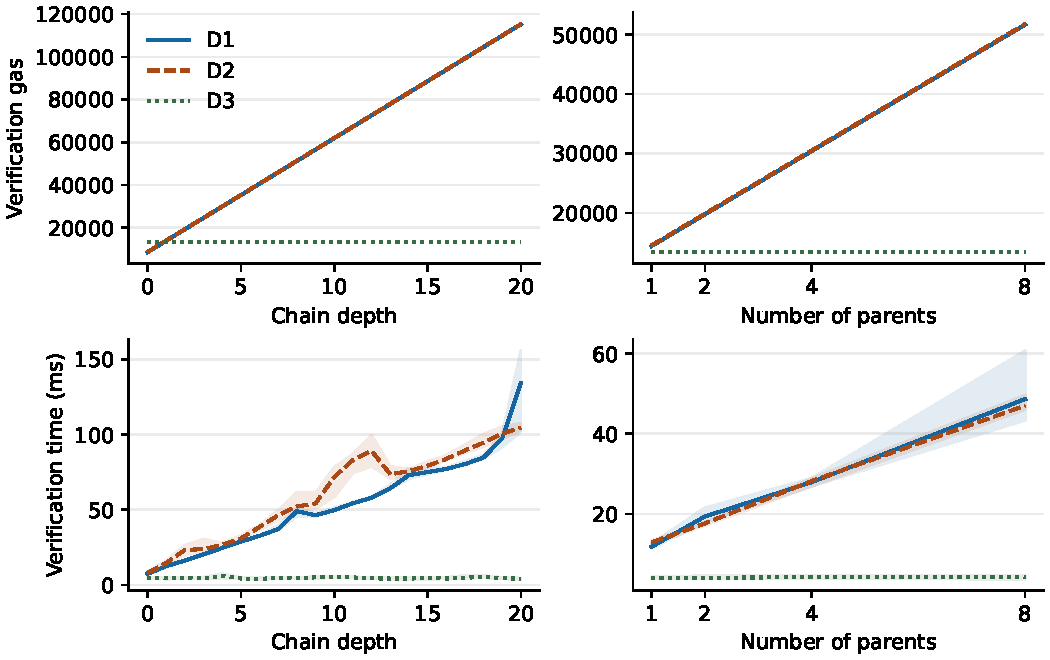
\includegraphics[width=0.94\textwidth]{synthetic_scaling.pdf}
\caption{Synthetic verification scaling on Anvil. D3 uses batches of
one model to hold proof size fixed. Shaded bands show the interquartile
range of wall-clock observations. D1 and D2 gas curves nearly overlap.}
\label{fig:scaling}
\end{figure*}

Figure~\ref{fig:scaling} separates chain depth from parent fan-in.
D1 and D2 walk additional records as either workload grows, increasing
gas and local verification time. D3 reconstructs the target commitment
off-chain and checks the target's inclusion and attestation on-chain.
The measured on-chain call stays roughly constant at batch size one.
The wall-clock curves cover the measured synthetic range with records
available locally. The separate proof-export demo audits each ancestor's
inclusion and attestation as well.

\begin{table}[t]
\centering
\caption{Audit rejections over applicable cases. Clean rejections
are false positives.}
\label{tab:integrity}
\setlength{\tabcolsep}{3pt}
\begin{tabular}{lrrrr}
\toprule
Design & Clean & Weights & Dataset & Parent \\
\midrule
D1 & 0/2,317 & 2,317/2,317 & 2,317/2,317 & 2,279/2,279 \\
D2 & 0/2,317 & 2,317/2,317 & 2,317/2,317 & 2,279/2,279 \\
D3 ($k=1$) & 0/2,317 & 2,317/2,317 & 2,317/2,317 & 2,279/2,279 \\
D3 ($k=16$) & 0/2,317 & 2,317/2,317 & 2,317/2,317 & 2,279/2,279 \\
D3 ($k=128$) & 0/2,317 & 2,317/2,317 & 2,317/2,317 & 2,279/2,279 \\
\bottomrule

\end{tabular}
\end{table}

\begin{table}[t]
\centering
\caption{Admission rejections over sampled candidates.}
\label{tab:admission}
\setlength{\tabcolsep}{3pt}
\begin{tabular}{lrrrr}
\toprule
Design & Clean & \shortstack{Unknown\\parent} &
\shortstack{Unlisted\\dataset} & \shortstack{Unauthorized\\publisher} \\
\midrule
D1 & 0/100 & 100/100 & 0/100 & 0/100 \\
D2 & 0/100 & 100/100 & 100/100 & 100/100 \\
D3 ($k=1$) & 0/100 & 100/100 & 100/100 & 100/100 \\
D3 ($k=16$) & 0/100 & 100/100 & 100/100 & 100/100 \\
D3 ($k=128$) & 0/100 & 100/100 & 100/100 & 100/100 \\
\bottomrule

\end{tabular}
\end{table}

Table~\ref{tab:integrity} shows that each verifier accepted all clean
records and detected every tested alteration. Parent substitution covered
\ParentCaseCount{} of \AuditModelCount{} records (\ParentApplicability{}).
Table~\ref{tab:admission} shows that all configurations refused an unknown
parent. D2 and D3 also refused the unlisted dataset references and
unauthorized publishers. These results describe the supplied fixtures
and the configured policy. The Iris workflow independently verified the
preserved files against immutable records for two versions.


\subsection{Public Sepolia replay}
We replayed a \SepoliaModels-model subset on both networks, using the
first models in registration order and adding a merge with its missing
ancestors. On-chain publisher identities matched across the pair. The
Anvil side used Cancun rules and the public Sepolia side used Glamsterdam.

\begin{table}[t]
\centering
\caption{Mean registration gas per model for the \SepoliaModels-model
sample. Anvil uses Cancun and Sepolia uses Glamsterdam. Deployment
and D2 policy setup are excluded.}
\label{tab:sepolia}
\begin{tabular}{lrr}
\toprule
Design & Anvil & Sepolia \\
\midrule
D1 & 577,952 & 2,656,796 \\
D2 & 623,781 & 2,842,907 \\
D3 ($k=1$) & 80,128 & 259,798 \\
D3 ($k=16$) & 5,508 & 19,106 \\
\bottomrule

\end{tabular}
\end{table}

Table~\ref{tab:sepolia} preserves the registration ranking observed on
Anvil. D3 with larger batches uses the least registration gas per
model on both networks. Sepolia used more gas for
\SepoliaHigherGas{} of the \SepoliaPairs{} paired transactions, including
deployments and policy setup. Glamsterdam's gas schedule changes the
cost of state creation and other operations. The cross-fork comparison
combines the effects of the gas schedule and execution environment.
D3 attestation calldata can also differ because signatures bind to
the chain ID and anchor address.


\section{Limitations}
The benchmark uses one snapshot of a predominantly shallow model family
and a separate synthetic workload for deeper ancestry. Hugging Face
dataset hashes cover the declared dataset names. Records with no declared
dataset use a fixed sentinel that is accepted by the experimental
allowlist. External parents are treated as roots of the sampled graph.
The Iris example instead
verifies the bytes of a preserved training CSV and separately stored model
artifacts. A matching hash supports an integrity claim about the checked
input. Hub declarations and the act of registering a record provide no
independent evidence of the training process or legal ownership. The D3
audit depends on the attester's integrity and the availability of the
off-chain records and proofs. Local latency depends on the machine,
software versions, and RPC access pattern.

\section{Conclusion}
The local measurements show where each design puts the work. Direct
storage makes the ancestry available through the registry. Solidity
policy enforcement adds registration work and can refuse candidates
outside the configured policy. Attested Merkle batches reduce on-chain
registration work and storage while relying on a trusted policy
attester and the continued availability of the records and proofs.
All designs detected the controlled alterations in the saved workload.
An independent proof-bundle audit also checked a merged model and its
ancestors against the anchor after the replay exited.

\section*{Acknowledgements}
The authors used OpenAI Codex to review the project plan, assist with
implementation and validation, and prepare an initial methodology draft.
% Authors: review this disclosure and include any other AI assistance.

\end{document}
